\begin{figure}[t]
    \centering
    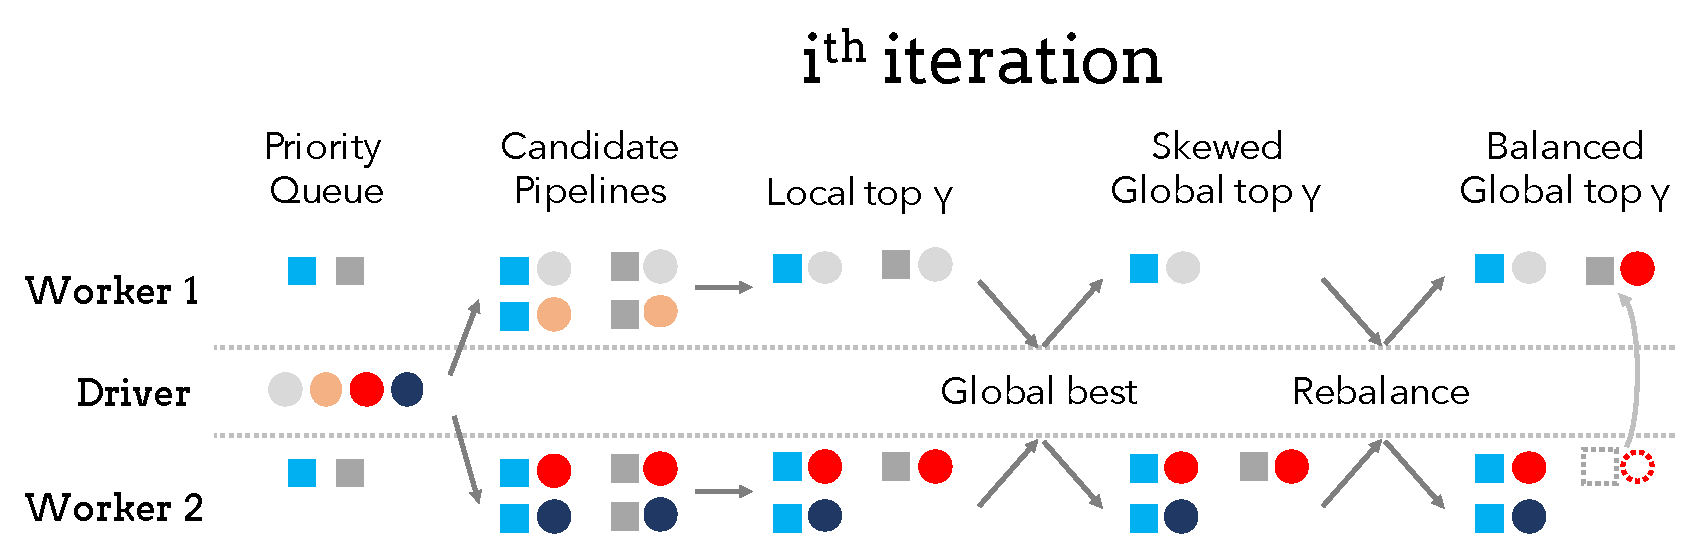
\includegraphics[width=\columnwidth]{figures/distributed.pdf}
    \caption{In each iteration, each worker starts with a subset of the priority queue (boxes).  The driver sends a subset of data transformations from $\Sigma$ (circles) to generate candidate programs (box-circles).  A series of synchronization points identify the globally top $\gamma$ candidates and redistributes them across the workers.   \label{fig:algo}}
\end{figure}

\section{Search Optimizations}\label{s:opts}
This section describes two important optimizations that allows \sys to generate cleaning programs in comparable runtimes as specialized systems.

\subsection{Parallelization}\label{s:parallel}
Composing and evaluating $Q(p'(R))$ is the single most expensive operation in the search procedure.   We now discuss how we parallelize its evaluation in shared memory and distributed settings, and the challenges when combining it with materialization.

\stitle{Shared Memory} In a naive, shared-memory implementation, we execute all expansions for a given $p\in P$ in parallel.  We materialize $p(R)$ in memory, and evaluate the quality of each $p' = p\circ T\ |\ T \in \Sigma$ in parallel using a  thread pool.  Each thread drops a given $p'$ if its quality is lower than $\gamma\times$ the maximum quality from the previous \texttt{WHILE} iteration or the local thread.  At the end of the \texttt{WHILE} iteration, the threads synchronize to compute the highest quality, and flush the remaining candidates using the up-to-date quality value.  The output of each $p'(R)$ can be retained or discarded using any cache replacement policy.  Our implementation uses Ray~\cite{ray} to schedule and parallelize the tasks.

\stitle{Distributed}
In the distributed setting, we do not have access to fast shared memory and the communication costs of sharing intermediate relations $p(R)$ can be impractical.  Thus, each worker is given a subset of candidate programs to locally evaluate and prune, and the main challenge is to reduce task skew through periodic rebalancing.  We use a worker-driver model with $j$ workers (\Cref{fig:algo}).

Let $P^{next} = P\times \Sigma$ be the set of candidate programs (e.g., 
\includegraphics[height=8pt]{figures/program.pdf}) to evaluate in the current iteration of the search algorithm. For instance, $P=\{NOOP\}$ in the first iteration, so the candidates are the set of individual data transformations $\Sigma$.   The driver assigns the input relation $R$ and $\frac{1}{j}$ of $P^{next}$ to each worker.  In the figure, the driver assigns a subset of $\Sigma$ to each worker.  Each worker evaluates and computes the top-$\gamma$ candidates based on the best worker-local quality.   The worker runs and caches the parents of its assigned candidate programs (
\includegraphics[height=8pt]{figures/sq-blue.pdf}, 
\includegraphics[height=8pt]{figures/sq-grey.pdf}) to incrementally compute the quality function.
  
Note that the worker-local top-$\gamma$ candidates are a superset of the top-$\gamma$ global candidates because the best local quality is $\le$ the global best.   Thus the workers synchronize with the driver to identify the global best candidate and further prune each worker's top candidates.  At this point, all candidate programs are within $\gamma$ of the globally best candidate, but their distribution across the workers can be highly skewed.  \sys performs a final rebalancing step, where each worker sends the number of un-pruned candidates to the driver.  Workers with more than $\frac{1}{j}$ of the total number redistribute the extras to workers with too few candidates.  When redistributing, workers communicate directly and do not involve the driver (e.g., Worker 2 sends 
\includegraphics[height=8pt]{figures/program-greyred.pdf} to Worker 1).   If the total number is $<k$, then candidates are randomly chosen to be replicated.  Only the programs and their qualities are sent; the program results are re-computed by the receiving worker.  This ensures that the priority queue in the next iteration is evenly distributed across all workers.  

% The workers then communicate the quality of their best transformation. This can be used to reconcile the local materializations to only the global top-$\gamma$ set.  This set is not necessarily balanced, e.g., one worker might have almost all of the top transformations.  The next step is a balancing step, where each worker communicates the number of materialized expansions it currently stores.  The workers with more than $\frac{|O|}{j}$ materialized expansions  randomly select ones to evict, and the driver re-distributes these to nodes with too few materialized expansions.  This is done by communicated the transformation and the result is re-computed on the new worker.  If $|O| < k$, then expansions are chosen at random to be replicated.  The result of the reconciliation step is that all workers have an evenly distributed set of materialized expansions.

% \item \ititle{Next Round} After reconciliation, each worker is associated with a particular $o \in O$ (or a set of them). To parallelize, the driver must simply ensure that it assigns new expansions only to those workers that have materialized the parent.  The algorithm then repeats, expanding each node locally, and then reconciles the results.

% The best-first search algorithm also is amenable to parallelization. One can parallelize over the two inner for loops $O \times L$. Each expansion can be forked into its own thread. However, this actually makes the materialization described above a bit more challenging. We use Ray~\footnote{https://github.com/ray-project/ray} to implement the parallel search. 
% 
% \subsubsection{Shared Memory Parallelization}
% The most straight-forward case is when we have access to low-latency shared memory between the expansion threads. In each expansion round, the main thread will assign each expansion node to workers and they will evaluate a given transformation. Each worker will make a copy of $o(R)$ (the node it is expanding) into shared memory. 
% If the expanded transformation is within $\gamma$ of the best current result, then it will update the copy, otherwise delete it. 
% 







\subsection{Dynamically Learning Pruning Rules}\label{s:dynlearn}
To effectively search through the language of transformations, pruning heuristics are important, yet hand-writing such heuristics {\it a priori} is challenging.
We describe how such heuristics can be automatically learned during the cleaning process.

\stitle{Motivation}
The search algorithms in  most automatic data cleaning frameworks are carefully tuned for a specific quality function or class of quality functions. For example, the chase used in functional dependency resolution does not make an edit to the table unless it enforces at least one tuple's FD relationship.    Similarly, in entity matching problems, one restricts the search to only matching tuples that are likely to be similar based on some similarity metric.
These can be viewed as search pre-conditions that exploit the structure of the cleaning problem to a more tractable search space.
Note that these are not static optimizations: knowing how to prune the search space requires identifying and modeling the structure of the underlying data errors and how they interact with the data transformations.
% the underlying data or making strong modeling assumptions about the types of transformations used.

%\ewu{So you're not training based on how the quality function changes as a program gets longer?  If each training example is simply the program for a block, how many blocks does there need to be?  If the search process isn't doing a great job, does that mean the learned classifier will suck?}

\stitle{Approach}
When \sys executes the search algorithm on each block of data, it generates a cleaning program that optimizes the quality metric for that block.  In many cases, the dataset can be partitioned into a large number of blocks that each serve as sources of training examples for a learned pruning model.  Each transformation in a block's  cleaning program $p_b$ can be labeled as a positive training example in $\Sigma_b^+$, while all other transformations serve as negative examples $\Sigma_b^- = \Sigma - \Sigma_b^+$.
As \sys processes more blocks, the union of these training sets can be sufficient to train a classifier to predict whether a given transformation will be included in the optimal program.  In our approach, the prediction model $M(T): \Sigma \mapsto \{0,1\}$ is over the data transformations and not the data; is this sense, \sys learns static pruning rules in a dynamic fashion.    

% \sys executes the search on each block of data.  The result is a sequence of transformations to optimize the quality metric on that block.  Every transformation in this sequence can be treated as a positive training example $L^+$, and every transformation not in this sequence can be treated as a negative example $L^-$.  The idea is that if we apply the search to a sufficient number of blocks then we can train a classifier to predict whether a transformation will be included in the final sequence.  It is important to note that this prediction is over the transformations and not the data. 

Internally, \sys uses a Logistic Regression classifier that is biased towards false positives (i.e., keeping a bad search branch) over false negatives (e.g., pruning a good branch). This is done by training the model and shifting the prediction threshold until there are no False Negatives. 


\stitle{Featurization}
To use this approach, we use featurizers to transform each data transformation $T$ into a $k$-dimensional feature vector: \textsf{feat}: $T\mapsto\mathbb{R}^k$.
For example, recall the \texttt{find\_replace(NYC, NY, city\_code)} transformation in~\Cref{ex1}.
The expert is free to encode potential signals as part of the transformation.  For instance, the edit distance between the two literal parameters (e.g., NYC, NY) and an indicator vector to specify the attrbitue (e.g., city\_code).  

Notice that many data transformation can be modeled as a predicate that specifies which records to clean, target attributes to clean, and replacement values for those attributes.  Thus, the featurized transformation potentially allows a model to learn which records, which attributes, and what replacement values, are highly to contribute to the final cleaning program.  For instance, \sys may learn that \texttt{find\_replace} only makes sense for \texttt{city\_name}.  Similarly, it may learn that the replacement string should be similar in edit distance to the source string, and subsequently learn the appropriate edit distance threshould.


\stitle{Discussion} We believe this is one of the reasons why a simple best-first search strategy can be effective.  For the initial blocks, \sys searches without a learned pruning rule in order to gather evidence.  Over time, the classifier can identify systematic patterns that are unlikely to lead to the final cleaning program, and explore the rest of the space.  In fact, this incremental learning process can be viewed from an active learning perspective to further target the exploration towards programs that will best improve the classification model.  

A potential benefit of learning a pruning model for {\it data transformations} rather than relation instances is that it can potentially be reused or fine-tuned for new, but structurally similar, data cleaning problems. In this way, the model can be trained {\it across data cleaning problems} rather than across blocks within a single problem.    In addition, we speculate that across a sufficient number of cleaning problems, if they share a common set of data transformation, we may adapt a deep learning approach to automatically learn the features themselves.  


% For example, some columns might not be dirty and are not worthwile to clean.  In the example above, another observation could be that the source and target strings in the optimal sequence are very close in terms of string similarity (as opposed to arbitrary transformations).  If each of these operations was featurized with a single scalar that is the edit-distance between the two strings, then the classifier could learn a pruning threshold (i.e., not considering find-and-replace operations above that threshold).  

% Consider an alternative to a predefined search heuristic where we clean data in small blocks.  For the initial blocks, we search without a heuristic.  As we continuously perform the search, we train a classifier on these features to reject search branches that are not typically in the final solution.  This allows us to exploit any patterns in the literal parameters that repeatedly occur.



